\documentclass[11pt]{article}
\usepackage[margin=1in]{geometry}
\usepackage{graphicx}
\usepackage{booktabs}
\usepackage{longtable}
\usepackage{array}
\usepackage{tabularx}
\usepackage{float}
\usepackage{multirow}
\usepackage{caption}
\usepackage{subcaption}
\usepackage{amsmath}
\usepackage{amssymb}
\usepackage{siunitx}
\usepackage{xcolor}
\usepackage{hyperref}
\usepackage{url}
\usepackage{enumitem}
\usepackage{pdflscape}
\usepackage{ragged2e}
\hypersetup{colorlinks=true,linkcolor=blue,urlcolor=blue,citecolor=blue}
\setlength{\emergencystretch}{3em}
\newcolumntype{Y}{>{\RaggedRight\arraybackslash}X}
\newcolumntype{P}[1]{>{\RaggedRight\arraybackslash}p{#1}}
\title{Spatiotemporal Evolution of the Ridgecrest Inter-Mainshock Earthquake Sequence\\\large Grid-Based and Fault-Segment Diagnostics of Triggering Between the Mw 6.4 and Mw 7.1 Mainshocks}
\author{TRACE}
\date{}


% --- EarthLink enforced font settings (XeLaTeX) ---
\usepackage{fontspec}
\usepackage{xeCJK}
\usepackage{unicode-math}
\setmainfont{DejaVu Serif}
\setCJKmainfont{Noto Serif CJK SC}
\setmathfont{XITS Math}
\usepackage[htt]{hyphenat}
% --- end enforced font settings ---

\begin{document}
\maketitle

\begin{abstract}
This report investigates the evolution of seismic activation during the Ridgecrest sequence between the Mw 6.4 mainshock on 2019-07-04 and the Mw 7.1 mainshock on 2019-07-06, with emphasis on whether activation along mapped fault directions was synchronous, progressively staged, cascade-like, or more structurally complex. The implemented workflow combined two complementary analyses: (1) a \SI{1}{km} gridded onset analysis over a fault-bounded study region buffered by \SI{5}{km}, using \SI{30}{minute} bins and a sustained-activation onset rule; and (2) a mapped-fault segment framework in which earthquakes were associated to the nearest segment within \SI{3}{km} and segment activation was defined as the first \SI{30}{minute} bin exceeding 5 events (10 events per hour). The gridded analysis retained 4,713 inter-mainshock earthquakes, mapped them to 2,968 grid cells, and found 104 activated cells among 445 occupied cells. The fault-based analysis built 1,019 segments from 977 mapped polylines and associated 4,490 of 4,627 filtered earthquakes (97.0\%) to mapped fault segments, but only 24 segments met the strict activation threshold. Diagnostic metrics show that activation was not synchronous across the fault system: only 16.7\% of activated fault segments were triggered within 60 minutes of Mw 6.4 and only 25.0\% within 240 minutes, while the fault-segment activation interquartile range was 832.5 minutes. The combined evidence supports a mixed and structurally heterogeneous triggering pattern rather than system-wide co-activation. At the same time, the stringent segment threshold and sparse number of activated multi-segment faults limit the ability to establish a robust, systematized along-fault cascade law. Within the mapped-fault framework, the Mw 7.1 nearest mapped segment was not itself anomalously late-activated; however, that inference remains conditional on surface-fault representation and nearest-segment assignment.
\end{abstract}

\section{Scientific Objective and Scope}
The objective of this study was to investigate the spatiotemporal evolution of the Ridgecrest earthquake sequence specifically during the interval bounded by the Mw 6.4 and Mw 7.1 mainshocks, and to determine the style of triggering along the mapped fault system. The two primary scientific questions were:
\begin{enumerate}[label=(\arabic*)]
    \item Was earthquake activation along fault directions approximately synchronous across the system?
    \item If not, was activation staged, cascade-like along faults, or more spatially complex with cross-fault jumps and localized heterogeneity?
\end{enumerate}

The analysis window was strictly limited to the inter-mainshock interval from 2019-07-04 17:33:49.040000+00:00 to 2019-07-06 03:19:53.040000+00:00. Therefore, the report addresses only the evolution between the two mainshocks and does not infer pre-Mw 6.4 background behavior or post-Mw 7.1 development.

\section{Data, Study Domain, and Implemented Workflow}
\subsection{Input datasets}
The workflow used the relocated Ridgecrest earthquake catalog, the mainshock reference table, and mapped surface-fault polylines provided in the project context. The exact source files were:
\begin{itemize}
    \item Earthquake catalog: \url{<REPO_ROOT>/examples/ridgecrest/data/catalog_TRACE/TRACE_ridgecrest_relocated.csv}
    \item Mainshock reference events: \url{<REPO_ROOT>/examples/ridgecrest/data/catalog_TRACE/main_shock_events.csv}
    \item Fault traces: \url{<REPO_ROOT>/examples/ridgecrest/data/faults/ridgecrest_surface_faults.json}
\end{itemize}

Task 01 validated 84,474 catalog input rows, with zero missing required rows, zero duplicate removals, zero invalid numeric rows, and zero invalid time rows in the visible quality-control summary. These values are documented in the task output table \url{../outputs/01_grid_onset_analysis/tables/qc_summary.csv}.

\subsection{Workflow actually implemented}
The final interpretation rests on three implemented task groups.

\paragraph{Task 01: Grid-based onset analysis.}
The fault-bounded study region was buffered by \SI{5}{km} in all directions and discretized into \SI{1}{km} \(\times\) \SI{1}{km} cells. Local seismicity rates were constructed using \SI{30}{minute} bins. The implemented onset rule for grid cells was \emph{not} the same as the fault-segment rule; instead, a cell was assigned an onset at the first \SI{30}{minute} bin with count \(\ge 2\) and sustained support in subsequent bins, specifically as documented in the run-parameter table: candidate plus next bin \(\ge 3\), or candidate plus next two bins \(\ge 3\) with nonzero post-candidate activity. Parameters are preserved in \url{../outputs/01_grid_onset_analysis/tables/run_parameters.csv}.

\paragraph{Task 02: Fault-segment activation analysis.}
Mapped fault polylines were projected and discretized into short contiguous segments with a target length of \SI{1}{km}. Earthquakes from the filtered inter-mainshock catalog were associated to the nearest fault segment when the minimum distance was less than \SI{3}{km}. For each segment, a \SI{30}{minute} time series was built, and activation was defined as the first time bin exceeding 5 events per \SI{30}{minute}, equivalent to 10 events per hour. Parameters are documented in \url{../outputs/02_fault_segment_activation/tables/run_parameters.csv}.

\paragraph{Task 03: Triggering-style diagnostics.}
The diagnostic stage integrated the grid-cell and fault-segment products to quantify system synchrony, assess whether any major faults showed robust along-fault propagation, measure cross-fault complexity, and examine the activation history near the Mw 7.1 nucleation area. Parameters include a \SI{60}{minute} early window, a \SI{240}{minute} intermediate window, a \SI{3}{km} Mw 7.1 neighborhood radius, and a requirement of at least 8 activated segments on a major fault for robust propagation testing. These settings are recorded in \url{../outputs/03_triggering_style_diagnostics/tables/run_parameters.csv}.

\section{Evidence Overview and Principal Deliverables}
The report draws primarily on the task outputs listed in the project evidence index. Key tables include the gridded onset metrics, fault-segment activation summary, system synchrony metrics, cross-fault complexity metrics, fault classification table, Mw 7.1 neighborhood segment table, and event-count conservation table. Representative figures are shown in Figures~\ref{fig:overview}--\ref{fig:mw71}.

\begin{figure}[H]
    \centering
    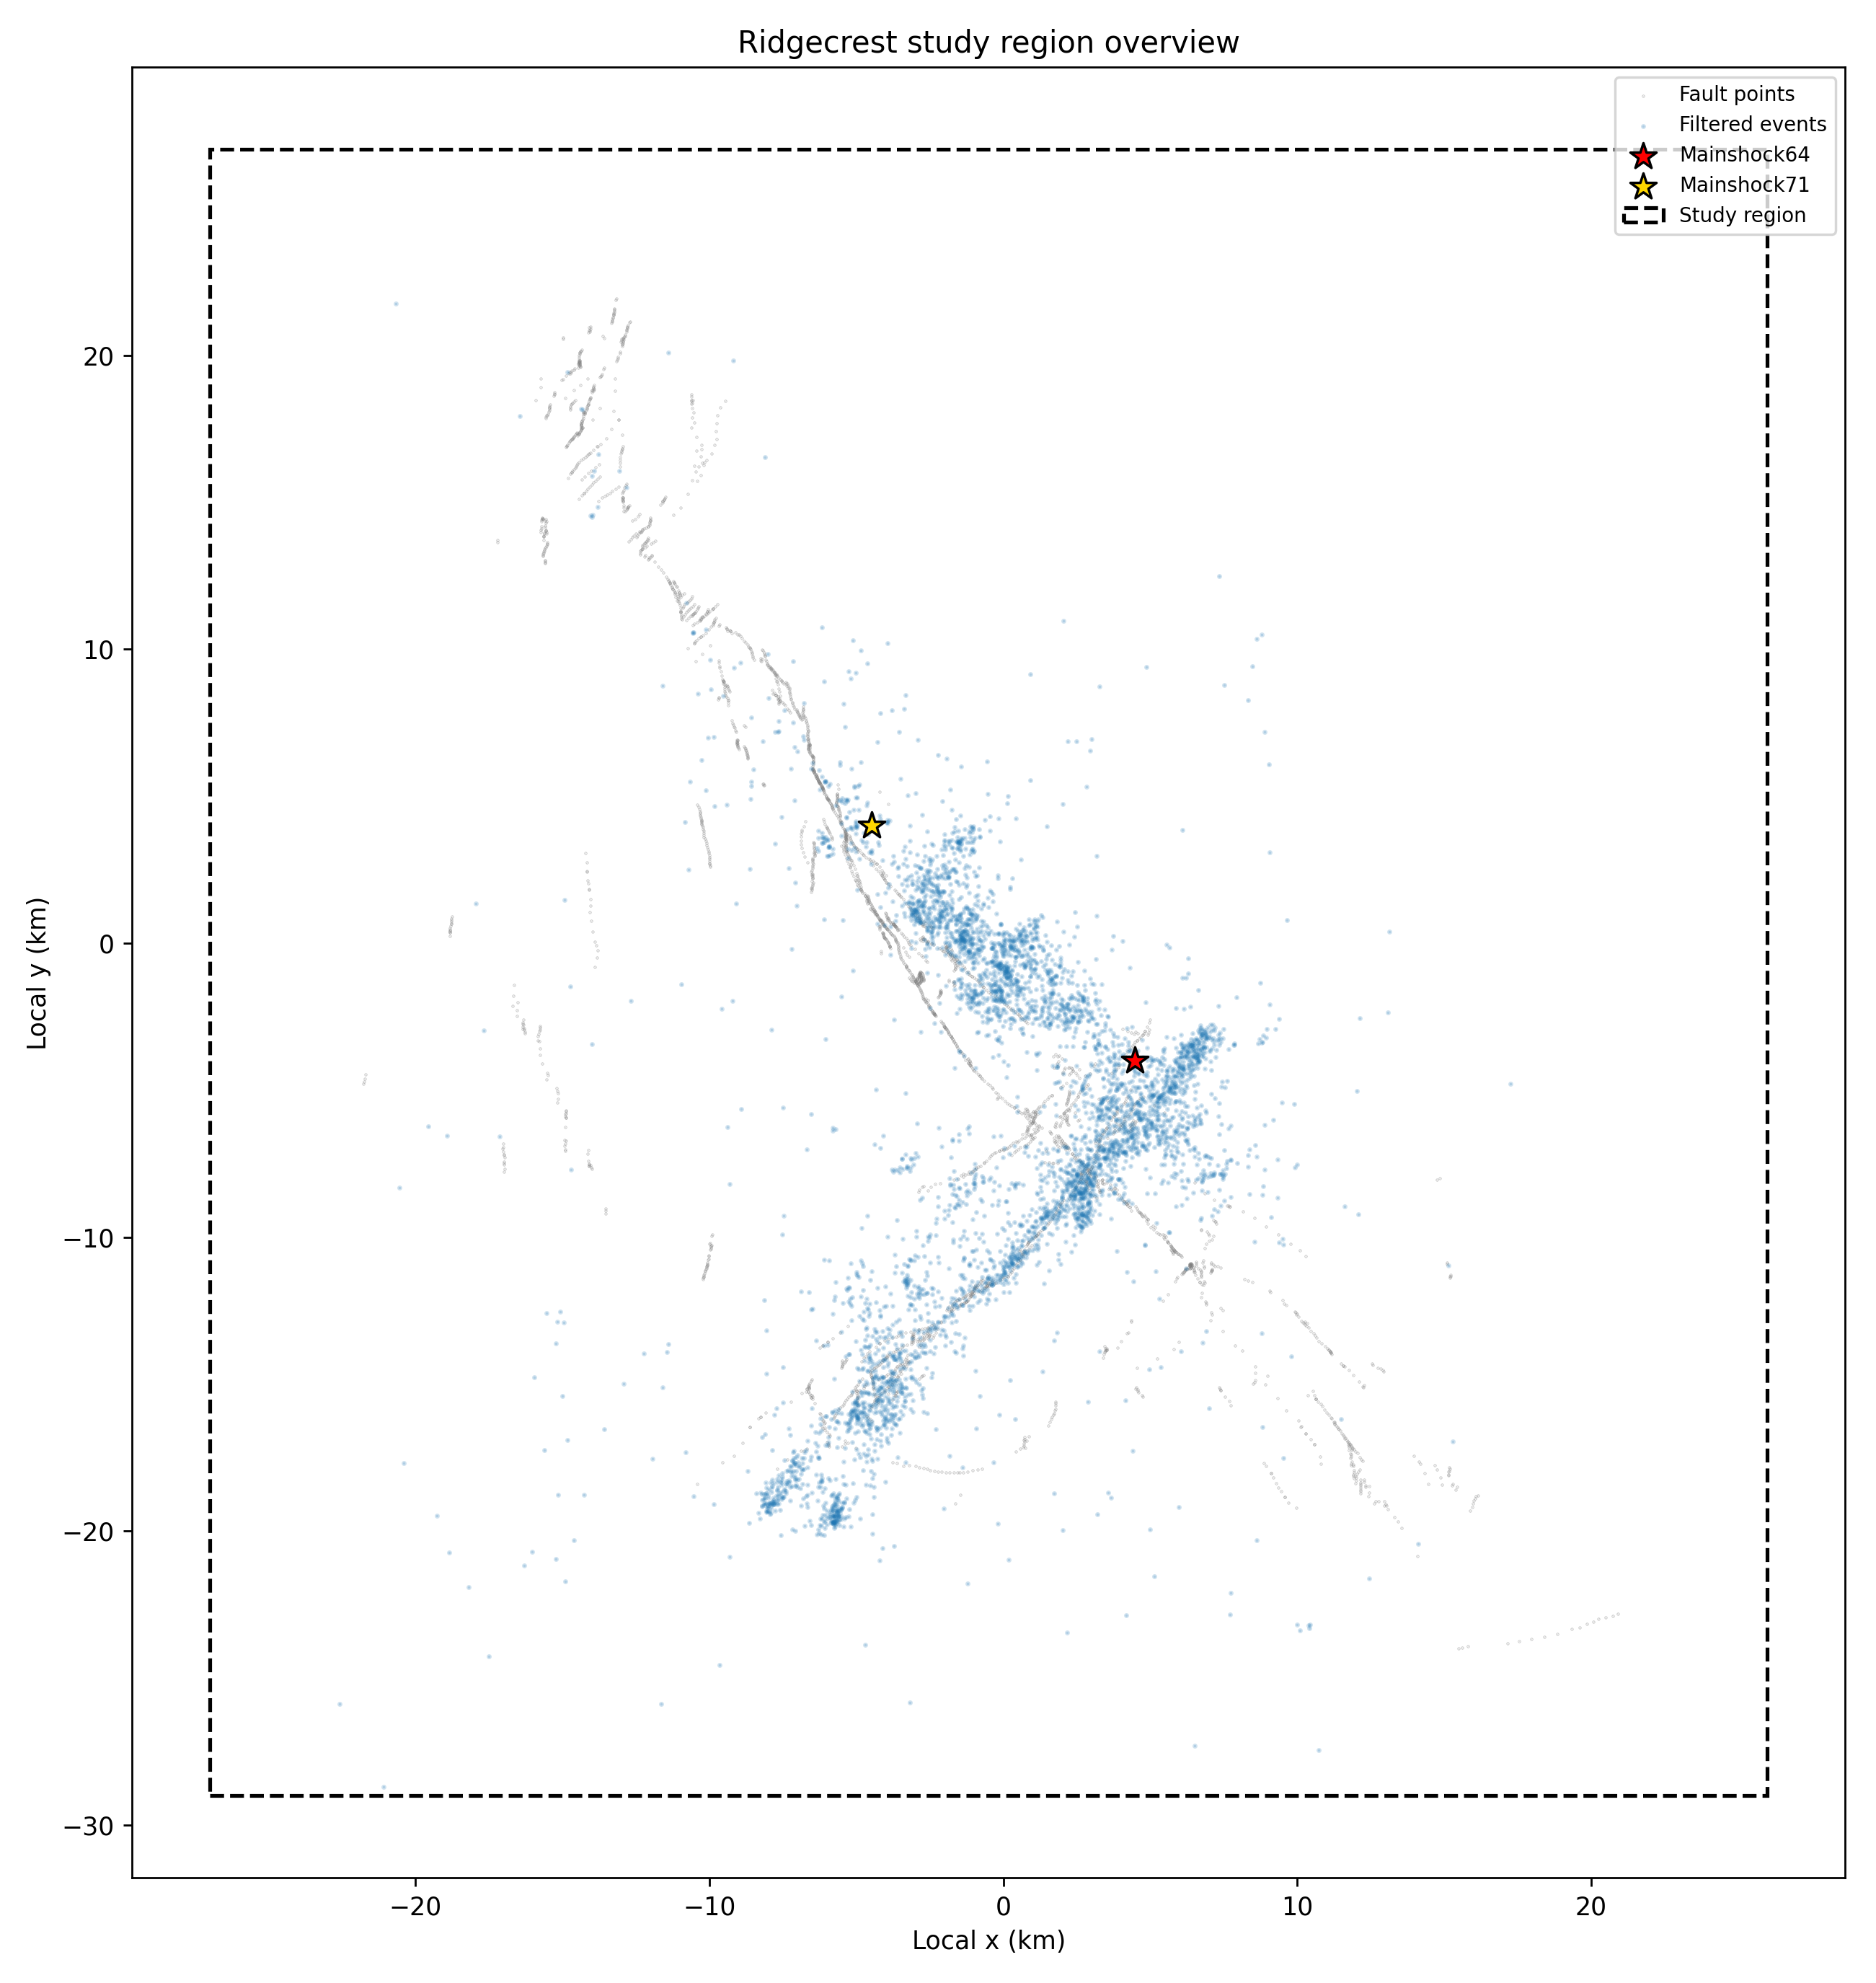
\includegraphics[width=0.8\textwidth]{../outputs/01_grid_onset_analysis/figures/study_region_overview.png}
    \caption{Study region overview for the Ridgecrest inter-mainshock analysis, showing the fault-controlled spatial domain used for the gridded onset framework.}
    \label{fig:overview}
\end{figure}

\begin{figure}[H]
    \centering
    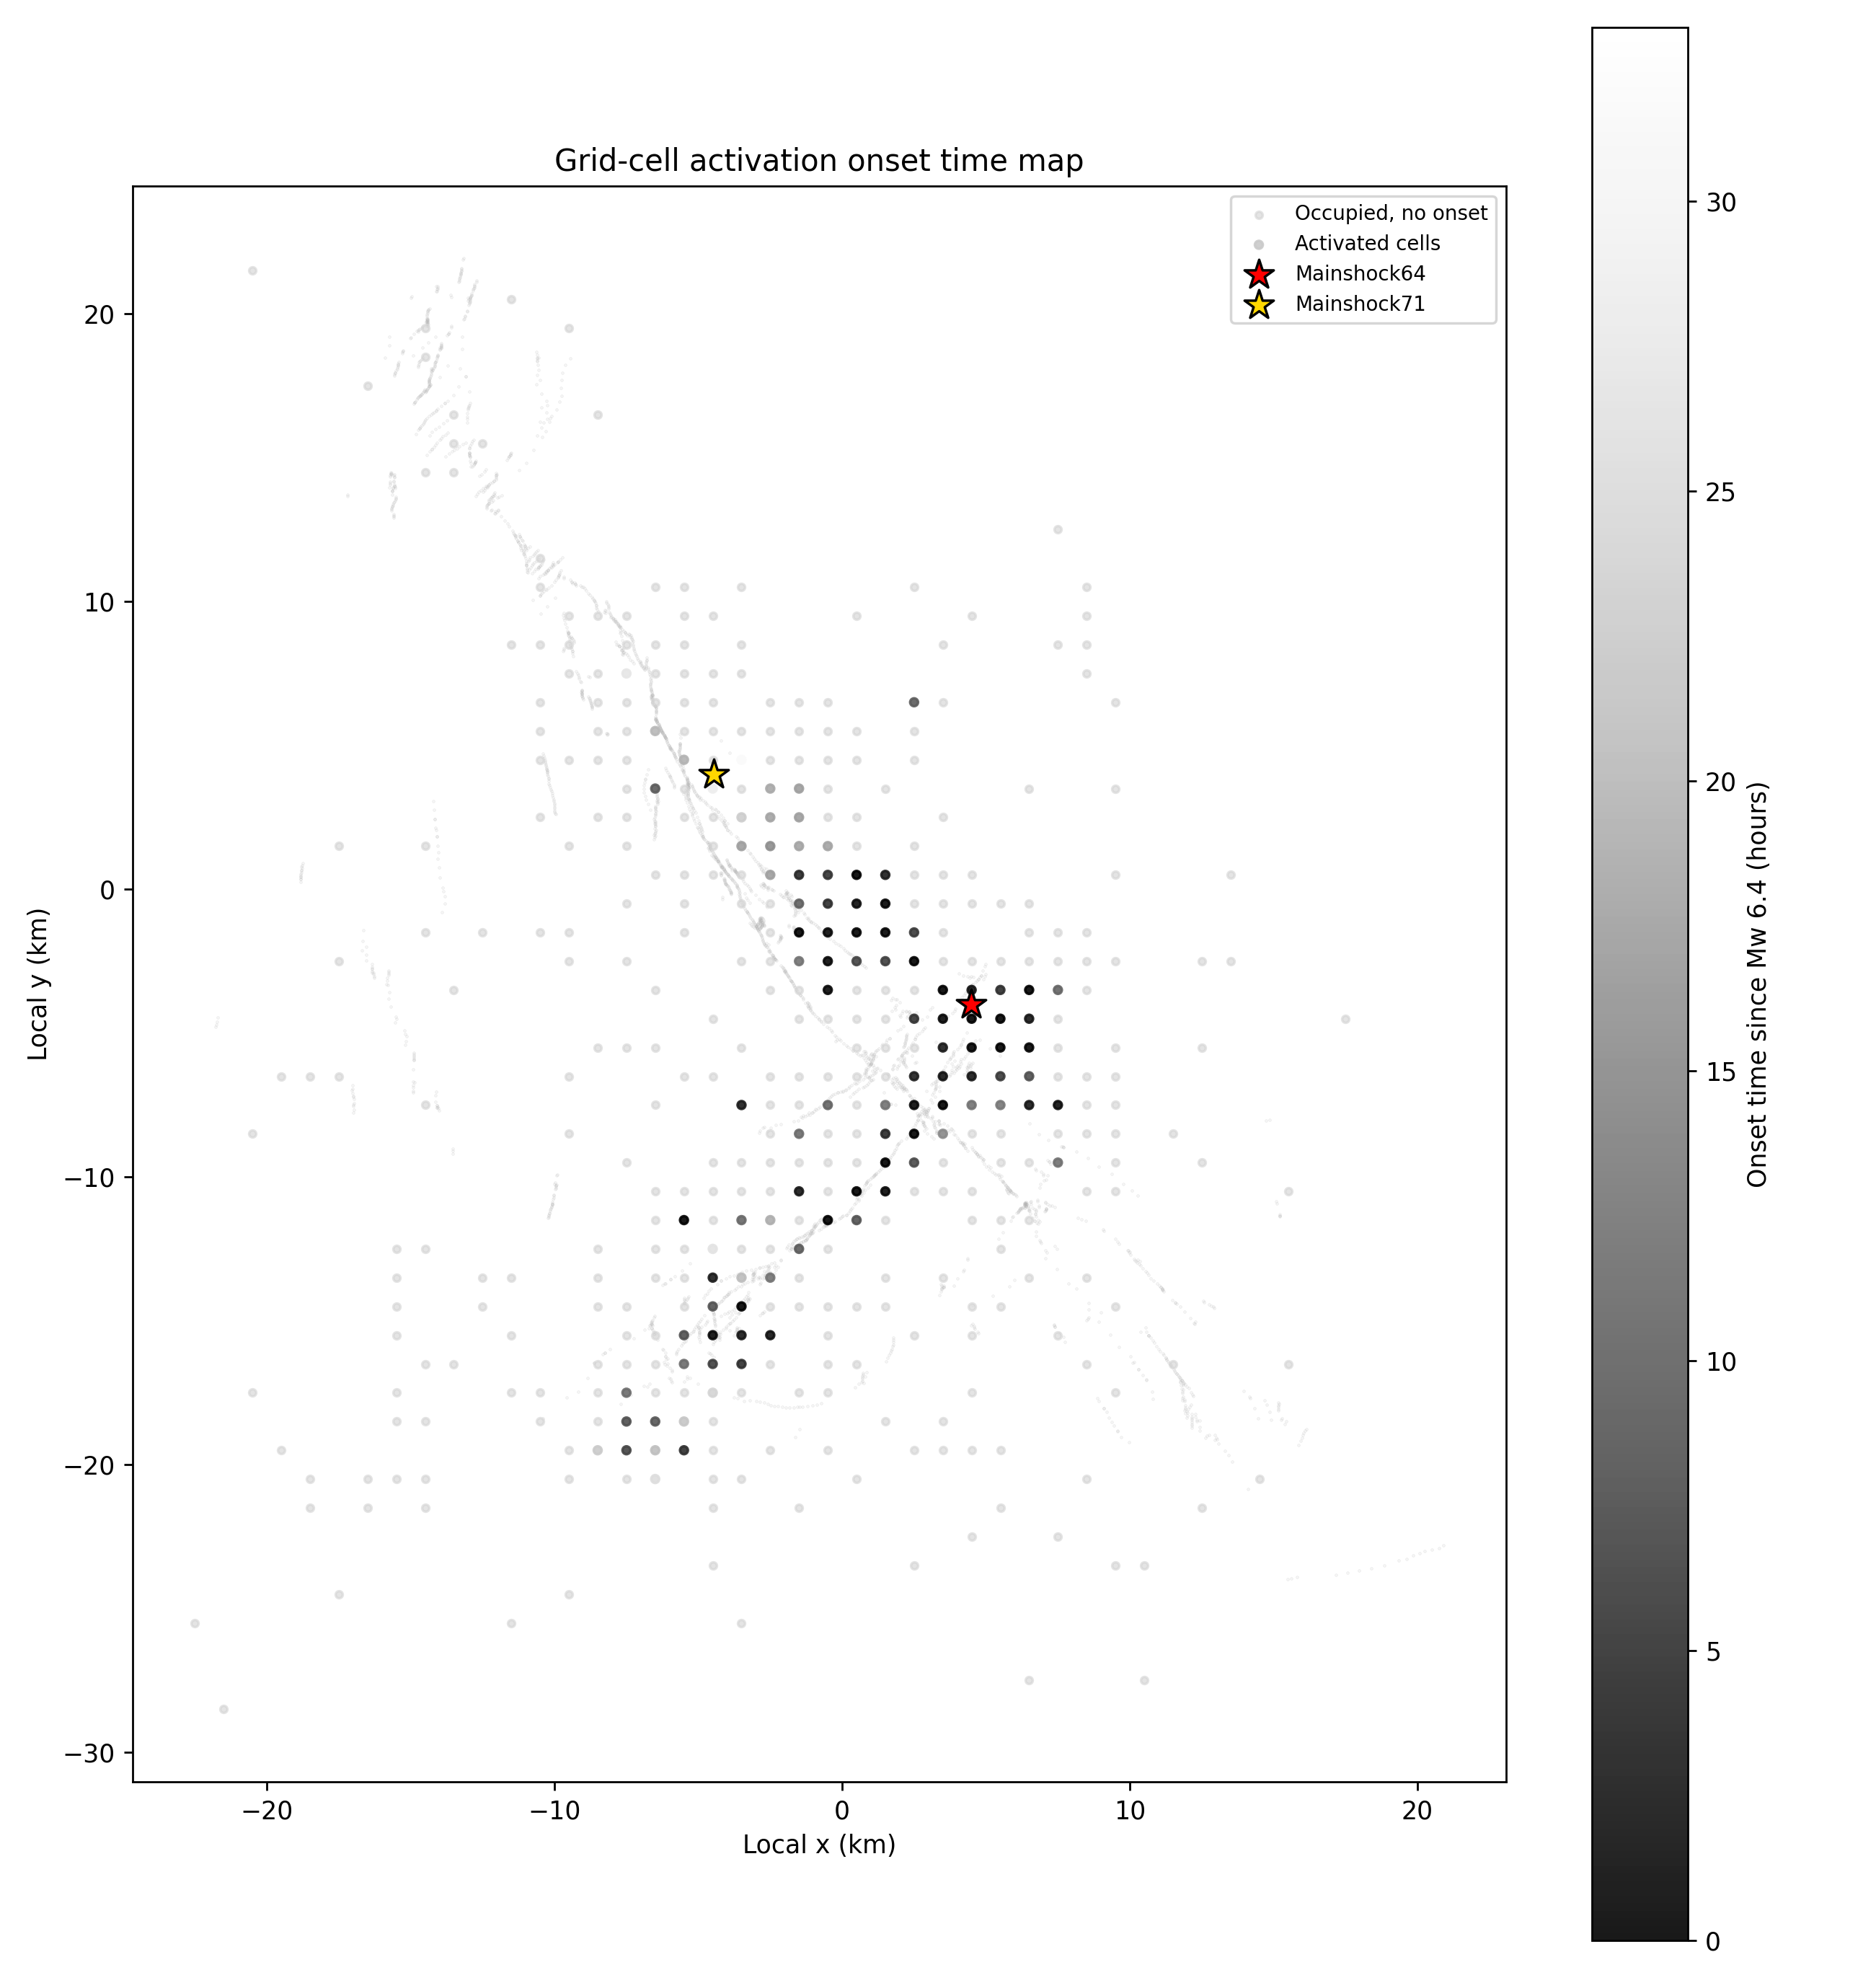
\includegraphics[width=0.8\textwidth]{../outputs/01_grid_onset_analysis/figures/grid_onset_map.png}
    \caption{Grid-cell onset map for the inter-mainshock interval. Darker tones represent earlier activation onset relative to the Mw 6.4 mainshock.}
    \label{fig:gridmap}
\end{figure}

\begin{figure}[H]
    \centering
    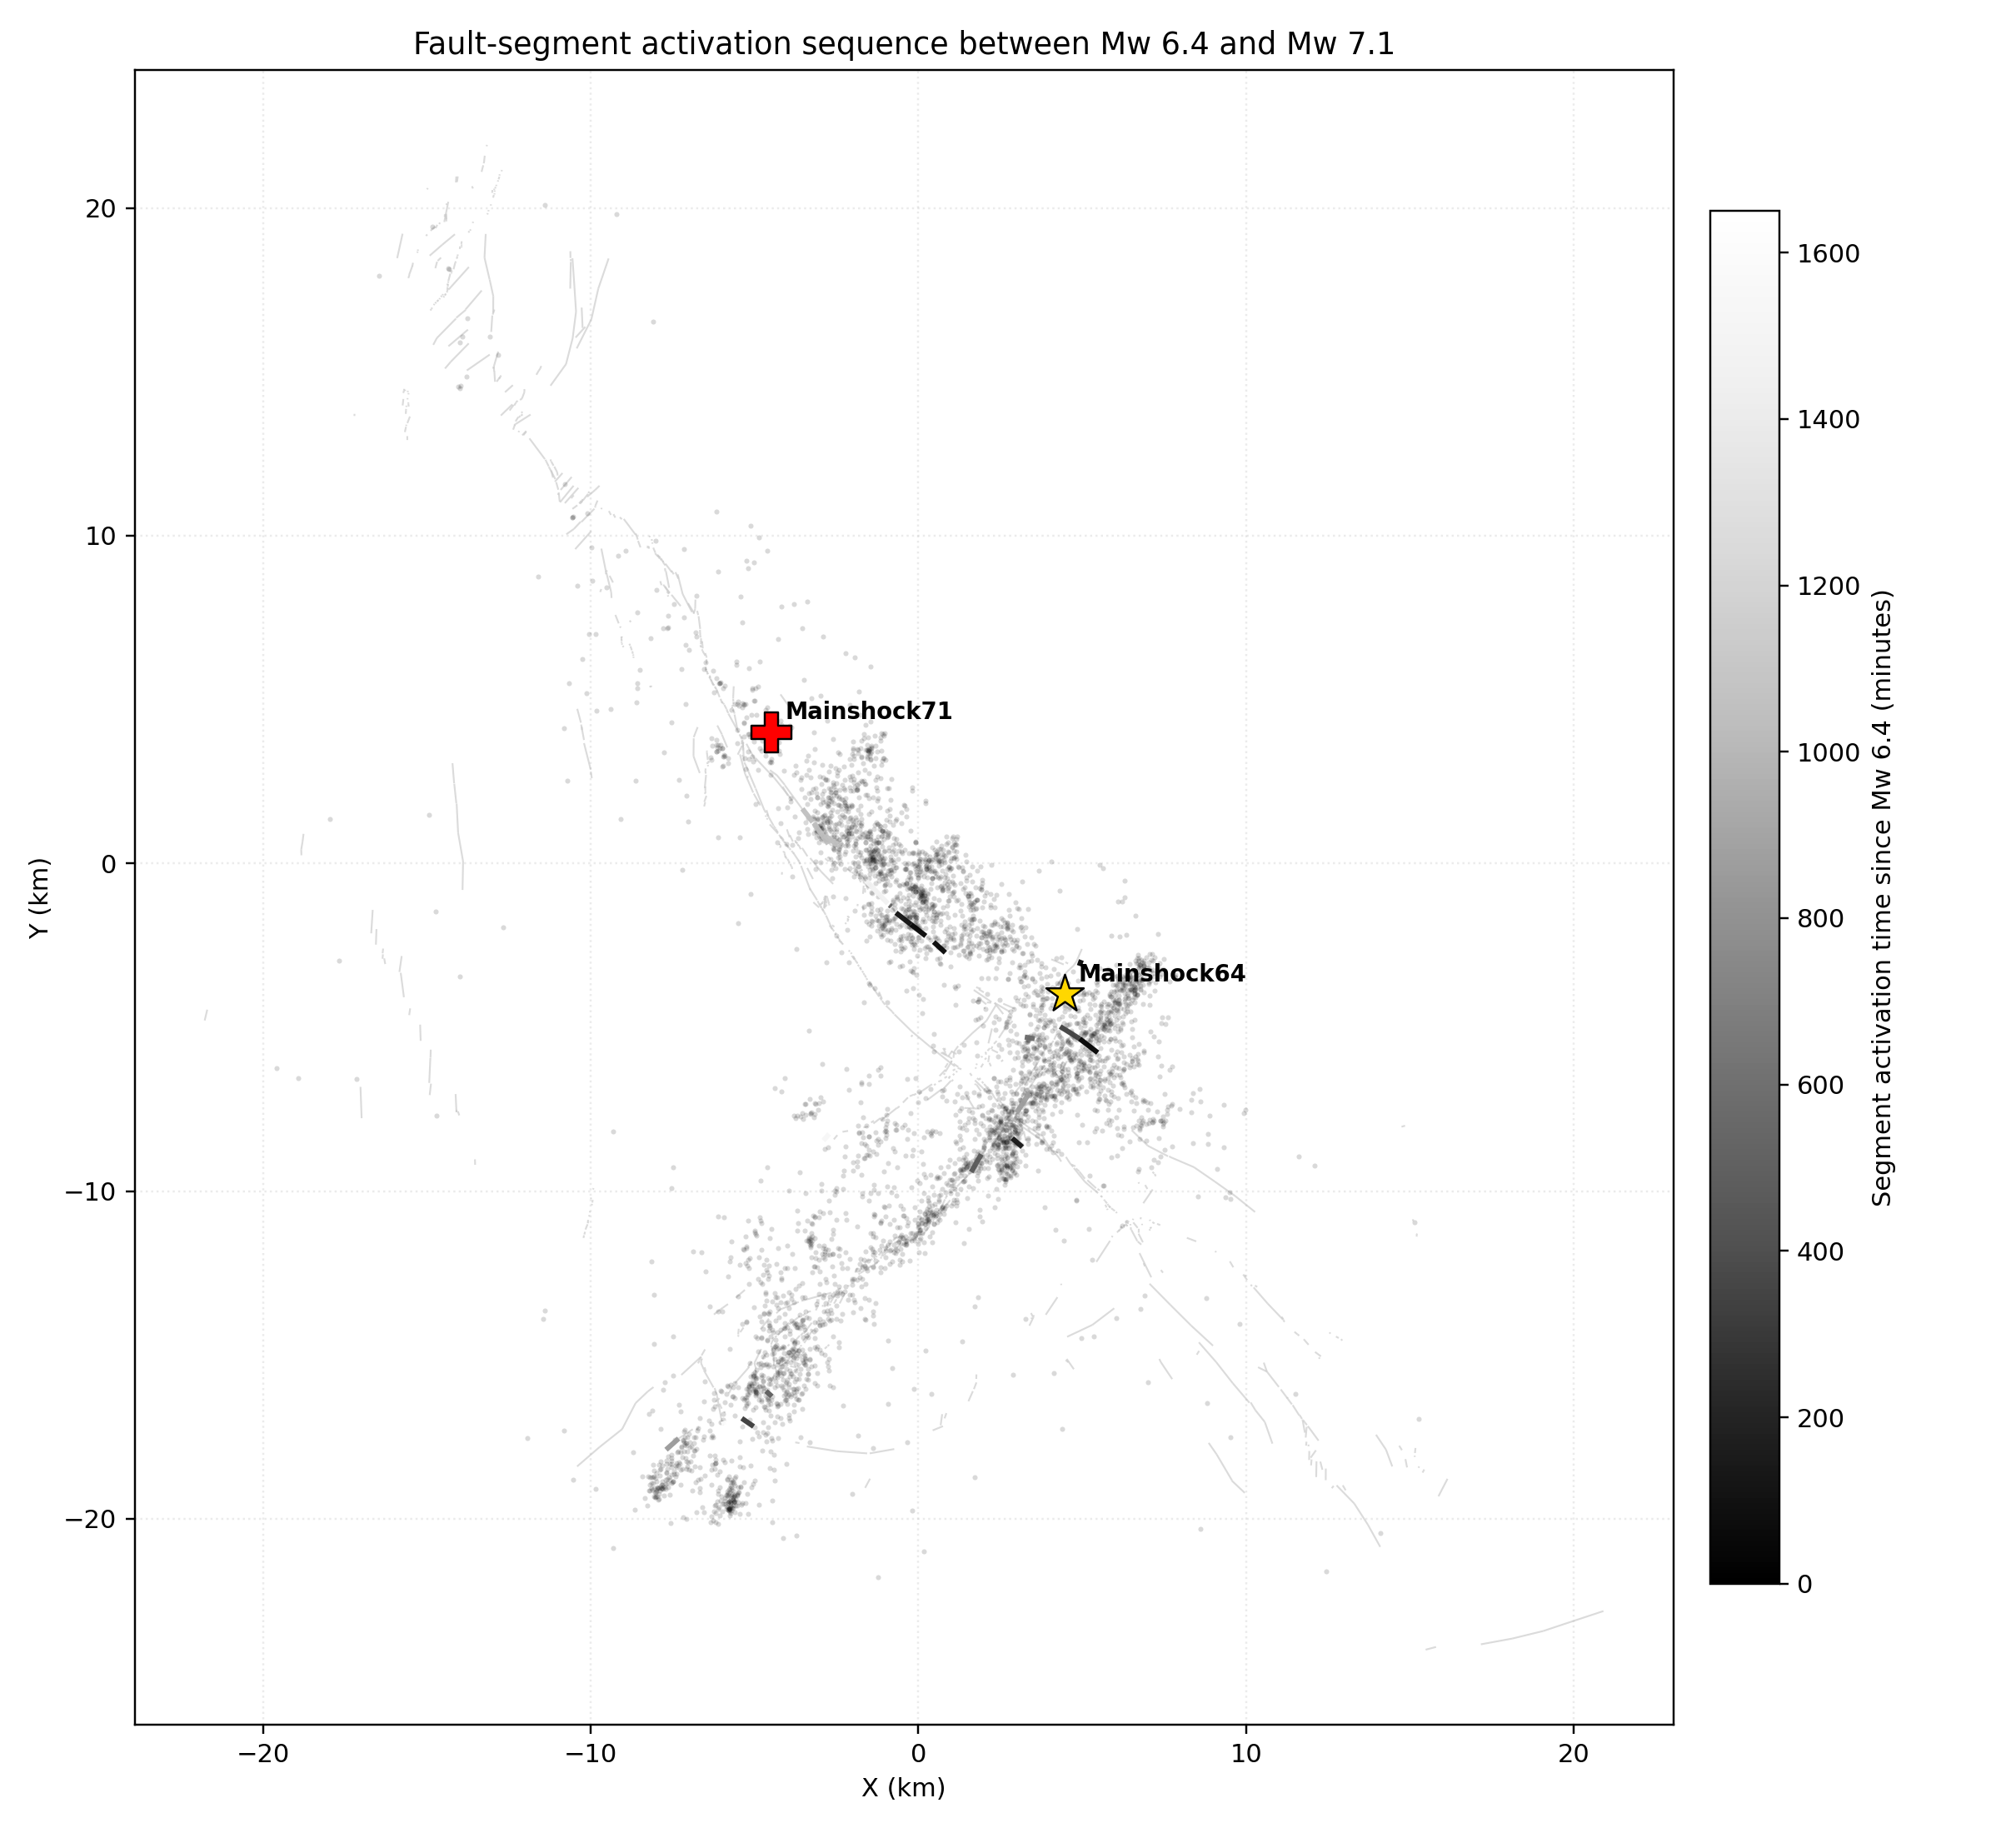
\includegraphics[width=0.8\textwidth]{../outputs/02_fault_segment_activation/figures/fault_segment_activation_map.png}
    \caption{Fault-segment activation map colored by activation time. This figure is central to evaluating whether activation progressed coherently along mapped fault directions or remained heterogeneous across the system.}
    \label{fig:faultmap}
\end{figure}

\begin{figure}[H]
    \centering
    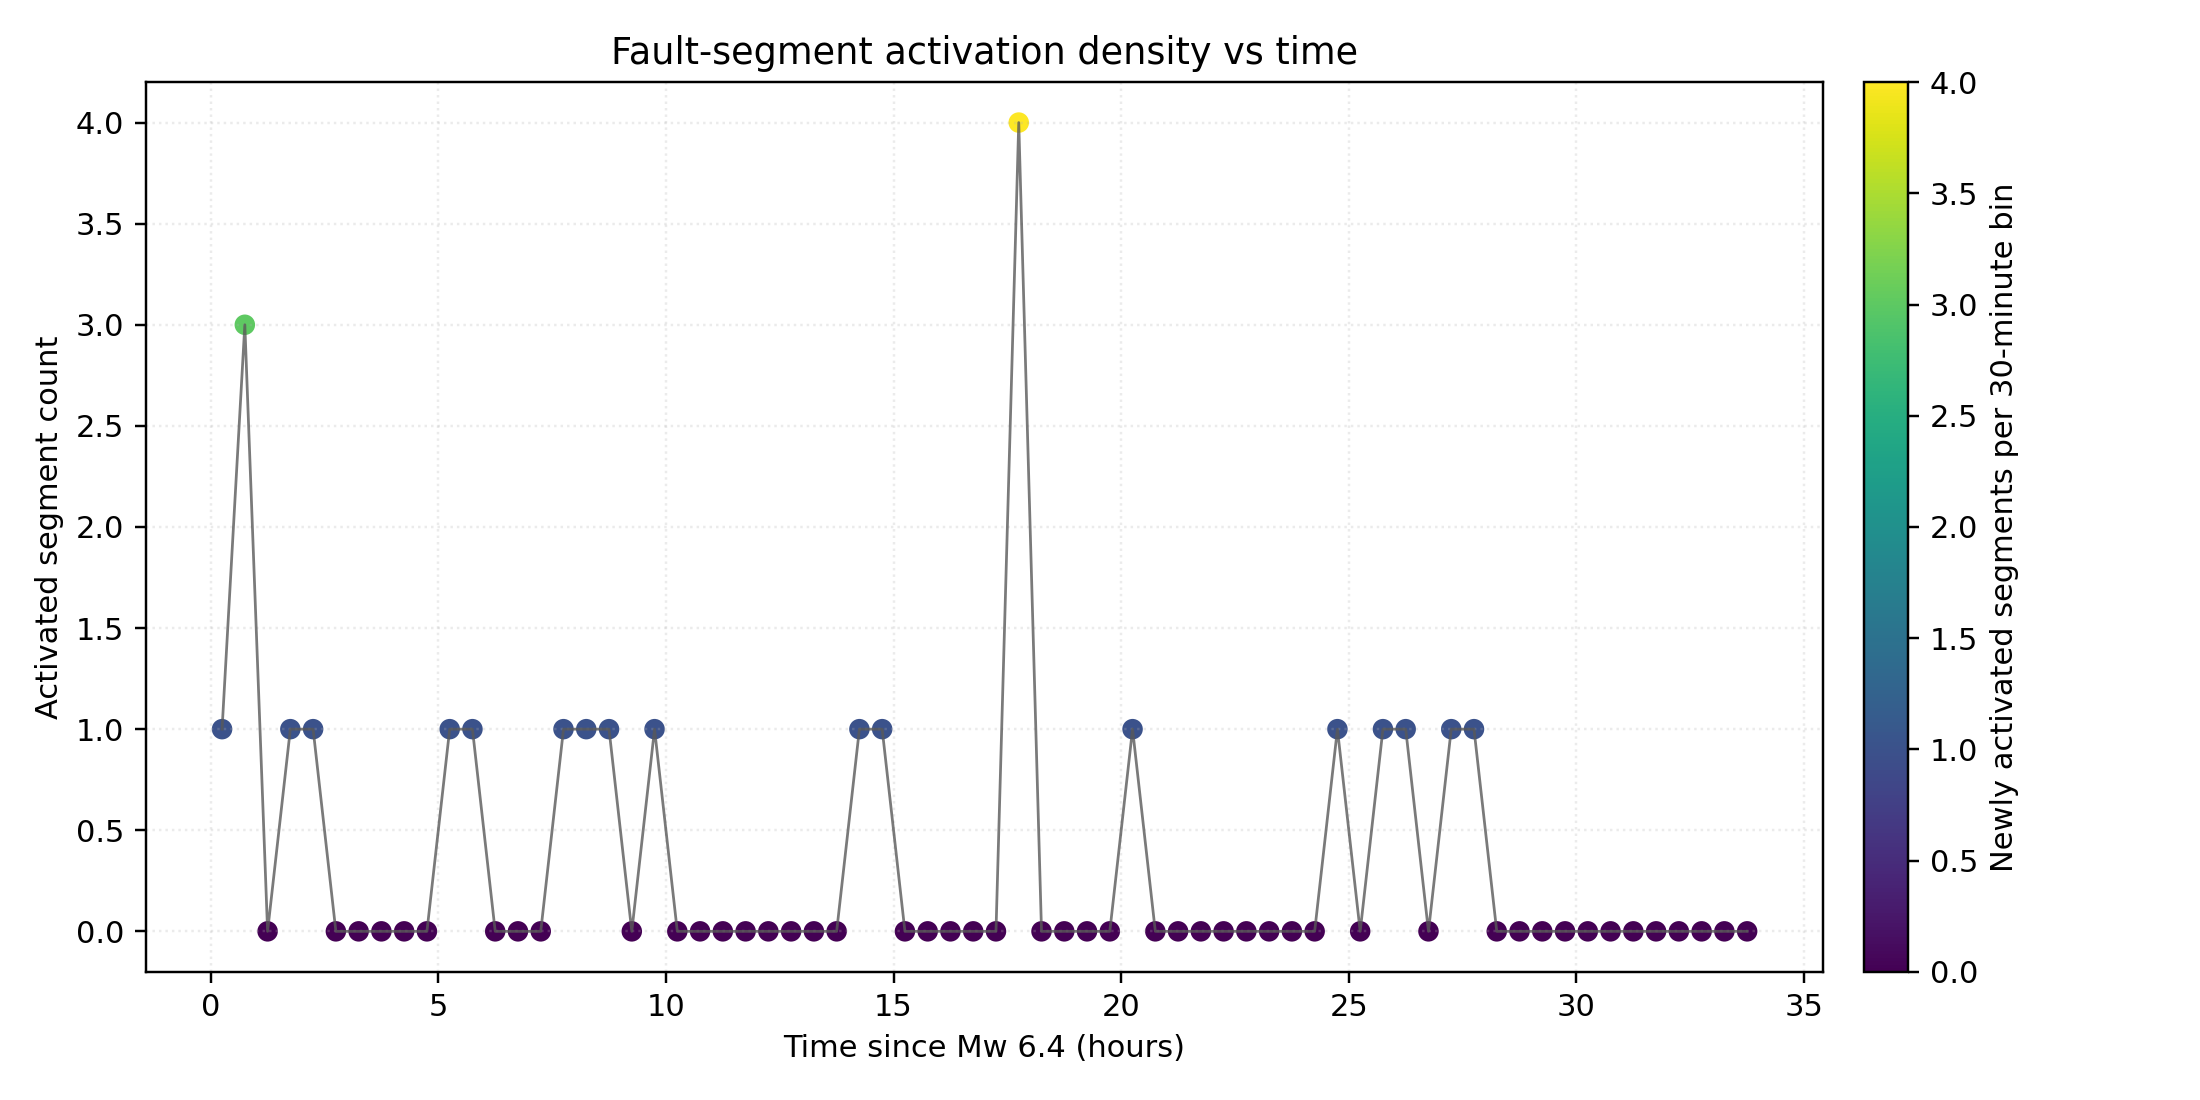
\includegraphics[width=0.8\textwidth]{../outputs/02_fault_segment_activation/figures/fault_segment_activation_density_vs_time.png}
    \caption{Temporal density of activated fault segments. Concentrated bands would support more synchronous behavior, whereas temporally broadened density supports staged or heterogeneous activation.}
    \label{fig:densitytime}
\end{figure}

\begin{figure}[H]
    \centering
    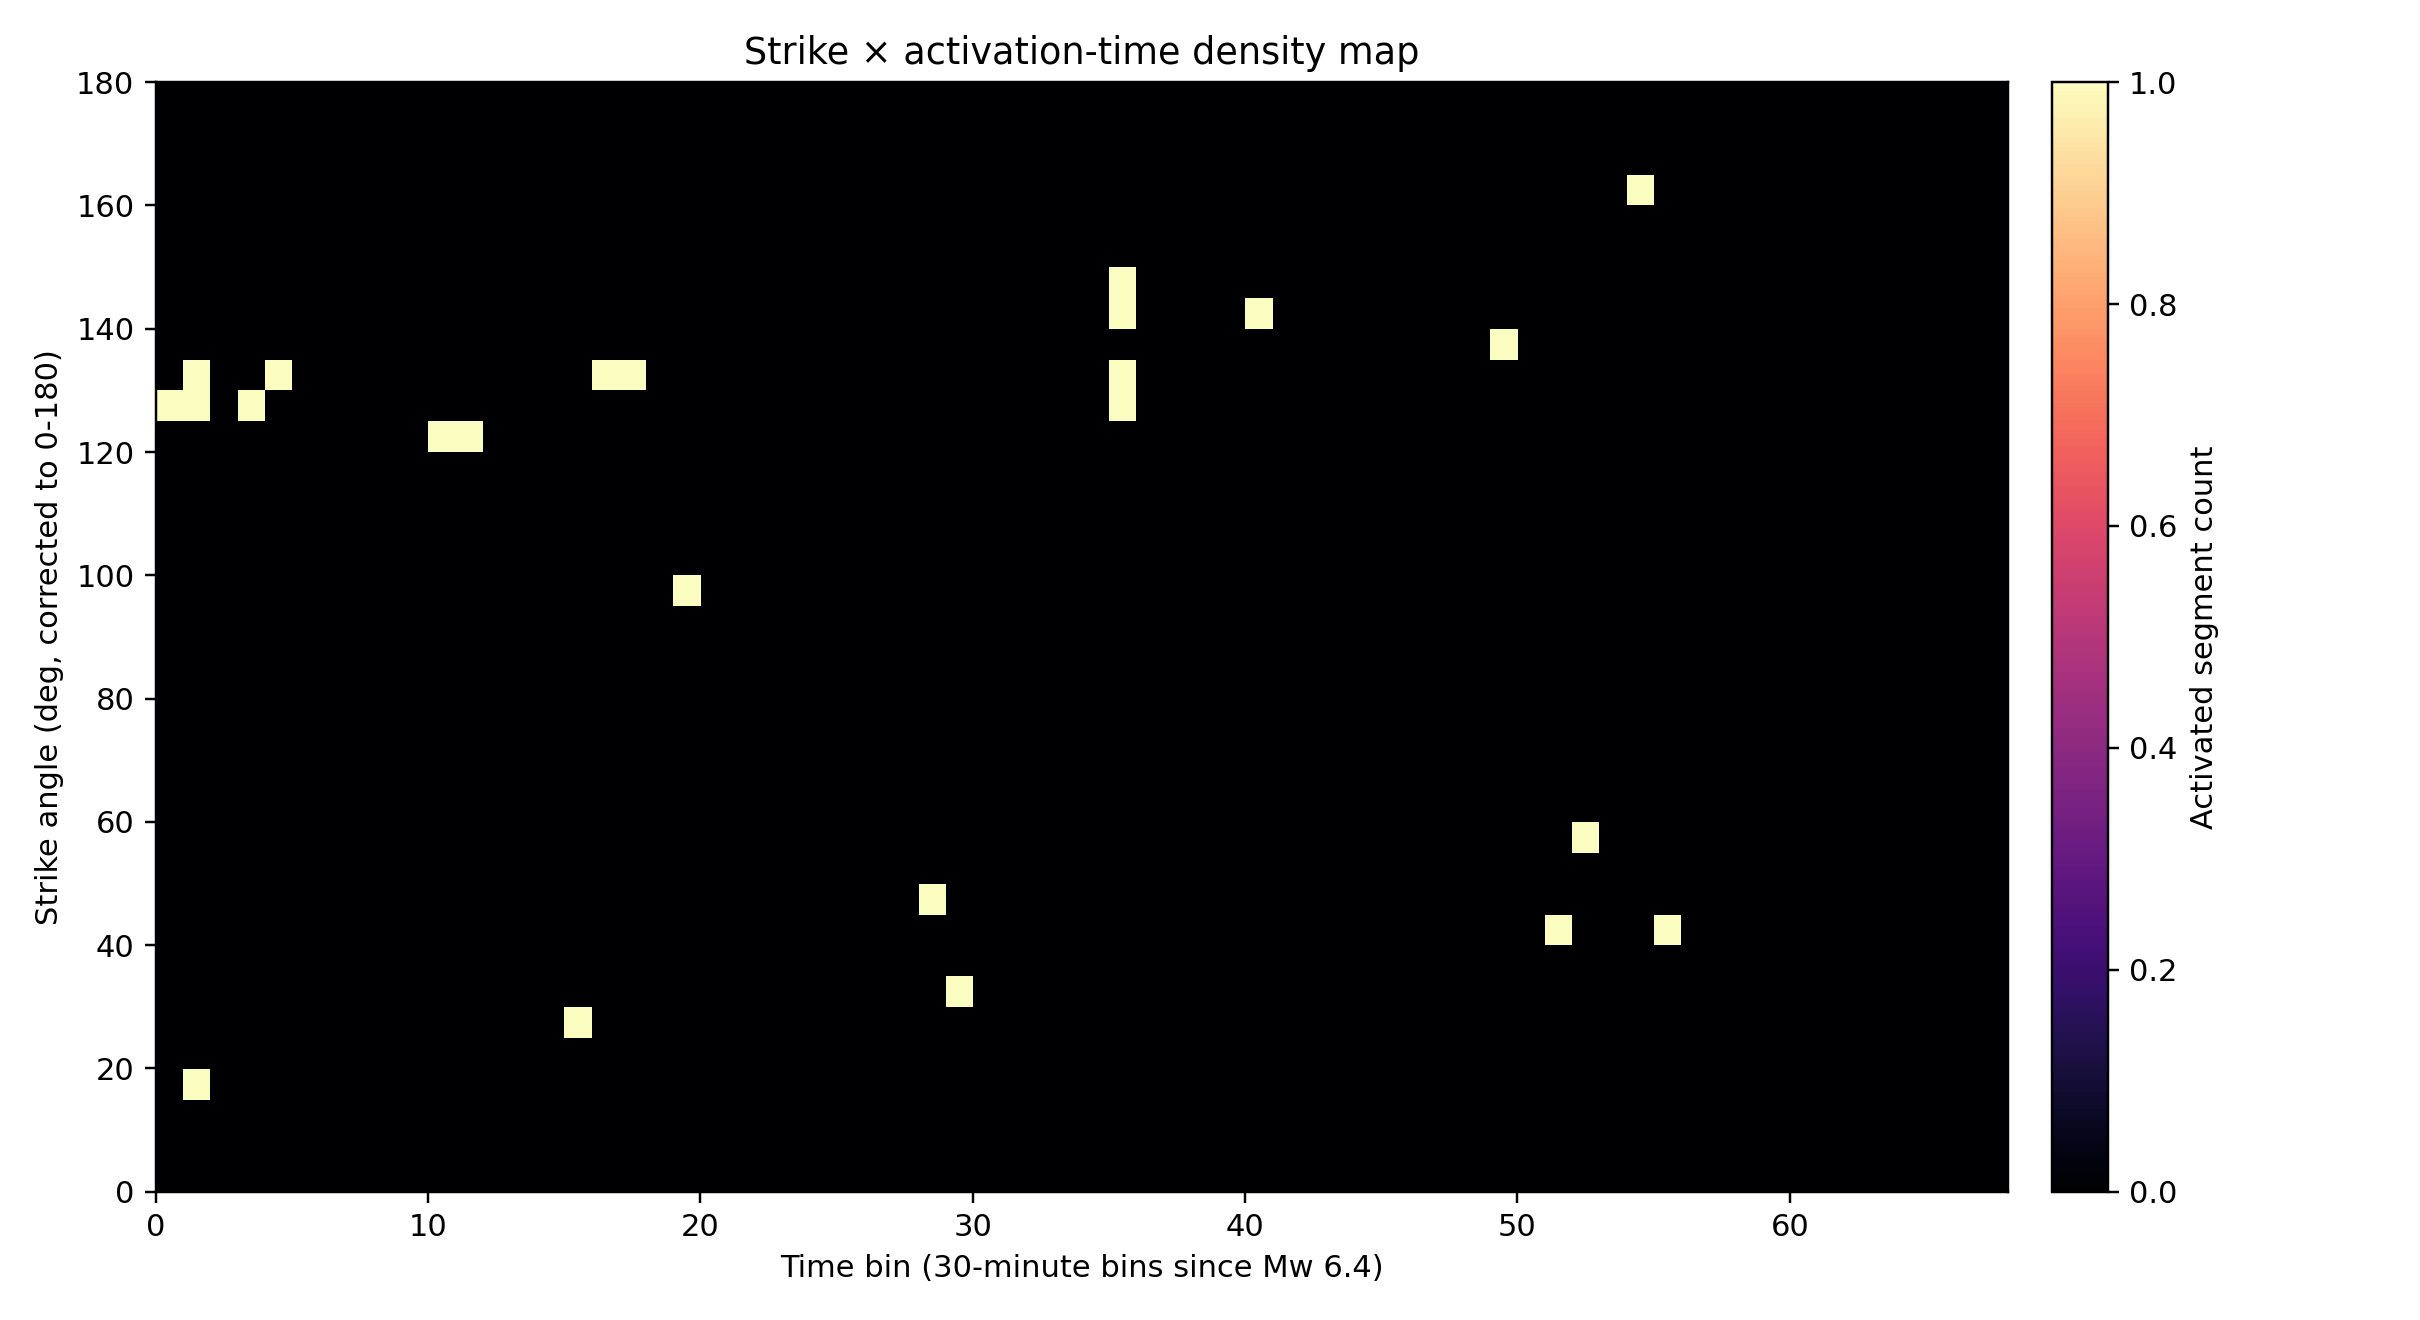
\includegraphics[width=0.8\textwidth]{../outputs/02_fault_segment_activation/figures/strike_activation_time_density.png}
    \caption{Strike-versus-activation-time density for activated fault segments. This view tests whether activation concentrated on a preferred fault orientation at specific times or jumped among orientations.}
    \label{fig:strikedensity}
\end{figure}

\begin{figure}[H]
    \centering
    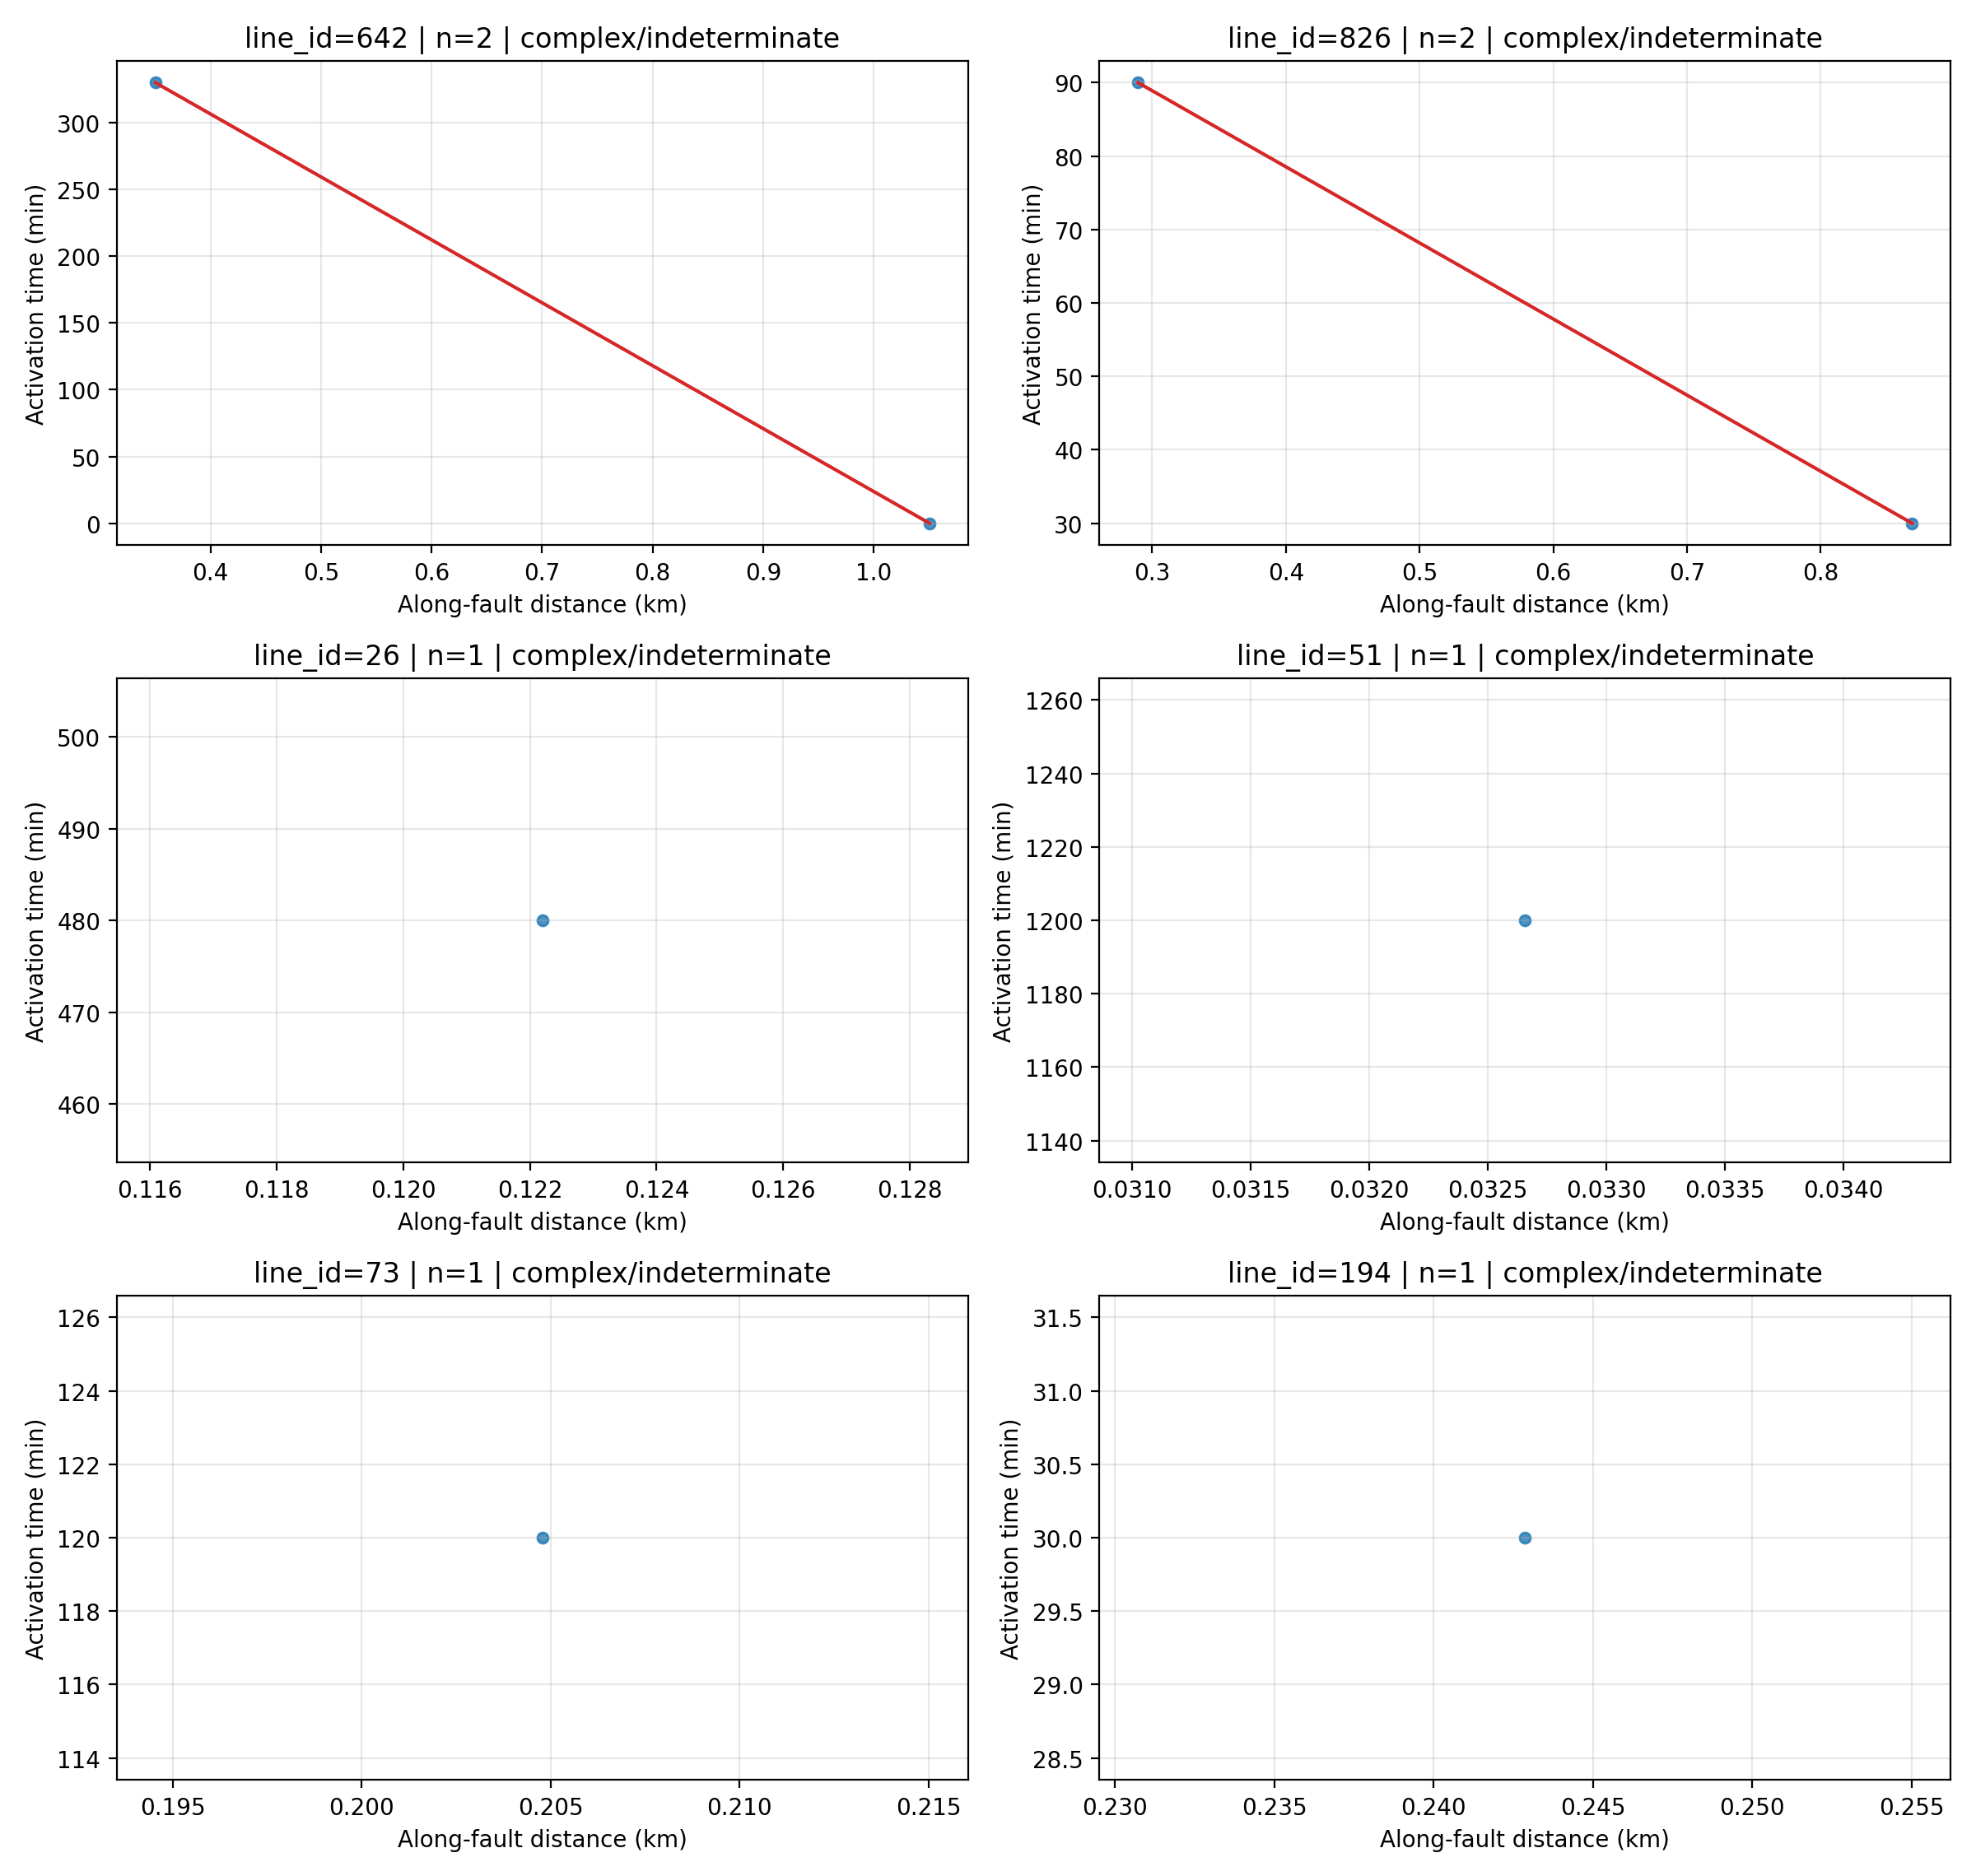
\includegraphics[width=0.8\textwidth]{../outputs/03_triggering_style_diagnostics/figures/along_fault_distance_vs_activation_time_major_faults.png}
    \caption{Distance-versus-activation-time view for major faults. The scarcity of faults meeting the eligibility criteria for propagation testing limits strong inference on systematized along-fault cascade behavior.}
    \label{fig:alongfault}
\end{figure}

\begin{figure}[H]
    \centering
    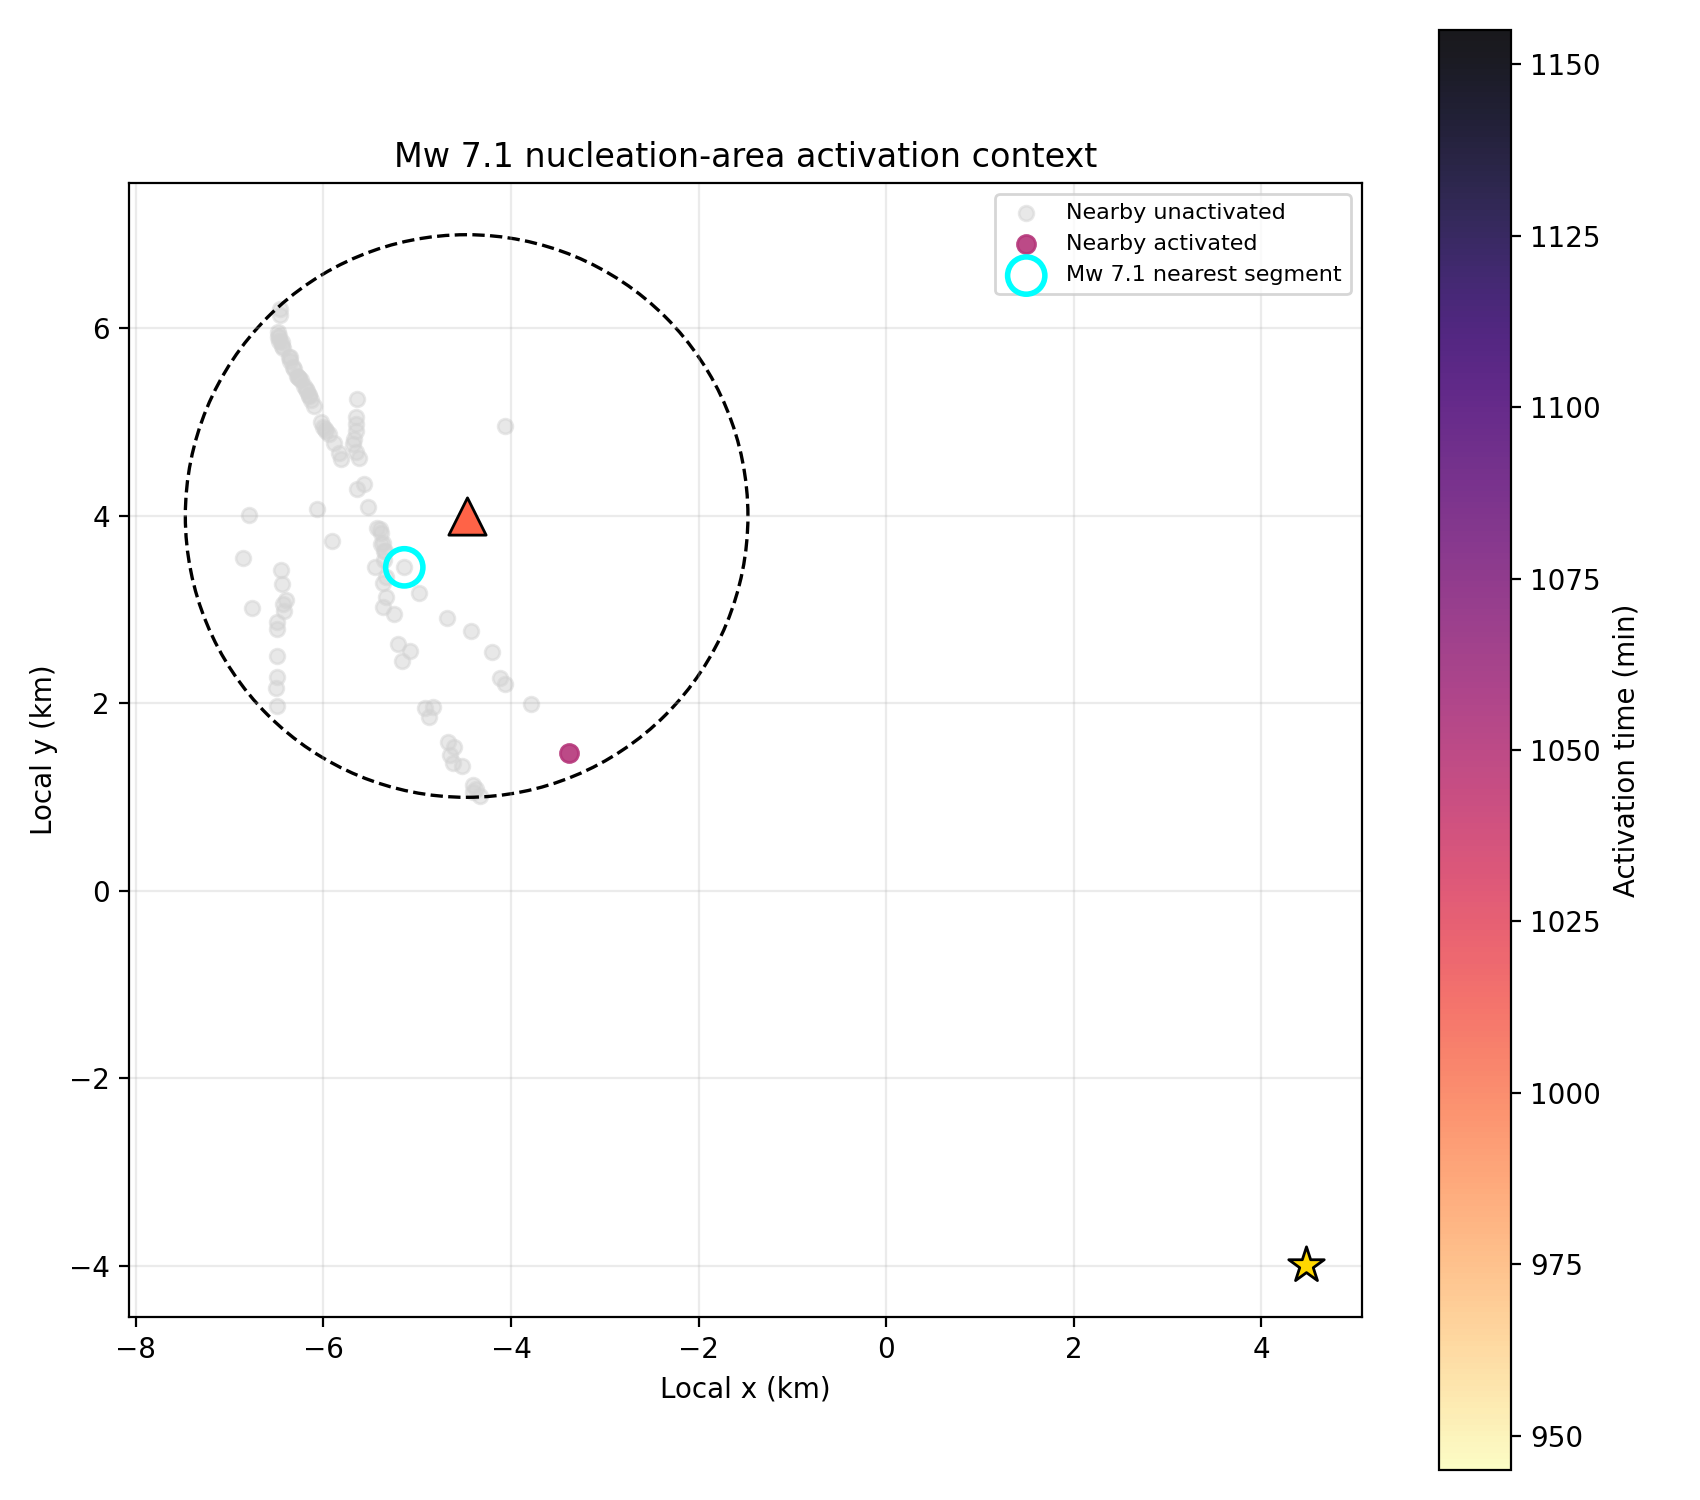
\includegraphics[width=0.8\textwidth]{../outputs/03_triggering_style_diagnostics/figures/mw71_nucleation_local_context.png}
    \caption{Activation context near the Mw 7.1 nucleation area, used to evaluate whether the nearest mapped segment activated anomalously late.}
    \label{fig:mw71}
\end{figure}

\section{Results}
\subsection{Grid-based onset patterns}
The gridded analysis established a reproducible onset framework for the inter-mainshock interval. According to the task claim and evidence tables, 4,713 earthquakes were retained between the two mainshocks and mapped onto 2,968 grid cells, of which 445 were occupied and 104 showed detectable onset under the sustained-count rule. The study therefore did not show universal or immediate activation across the occupied region.

Early activation fractions from the grid metrics were limited. In the task-level onset metrics table, the fraction of occupied cells activated within 30, 60, 120, and 240 minutes was 0.0449, 0.0607, 0.0719, and 0.0944, respectively, when normalized over all occupied cells. In the integrated synchrony table, where the denominator is the activated-cell subset, the fractions were 19.2\%, 26.0\%, 30.8\%, and 40.4\%, respectively. This confirms that activated cells were spread across time rather than concentrated immediately after Mw 6.4. The spatial pattern in Figure~\ref{fig:gridmap} likewise indicates distributed onset times rather than a single front-like activation sweeping the entire study region at once.

\subsection{Fault-segment framework and event association}
The fault-based workflow produced 1,019 discretized fault segments from 977 mapped polylines. The segment-length distribution, however, was much shorter than the nominal \SI{1}{km} target, with median length \SI{0.122}{km} and mean length \SI{0.222}{km}, as recorded in the Task 02 quality-control table. This means the fault backbone preserved mapped geometry but did not produce a uniform physical segmentation scale.

From 4,627 filtered inter-mainshock events entering the segment-association stage, 4,490 events (97.0\%) were associated to a nearest segment within \SI{3}{km}, leaving 137 unassociated events. The compact context reports a median event-to-segment distance of \SI{0.592}{km}, supporting the interpretation that seismicity was strongly fault-controlled in map view. However, the event-count conservation table shows that Task 01 retained 4,713 events, whereas Task 02 operated on 4,627 rows before association. This discrepancy was explicitly tracked in the workflow and should be read as a filtering-stage difference rather than an unacknowledged inconsistency; the documented counts are listed in Table~\ref{tab:counts}.

\begin{table}[H]
\centering
\caption{Event-count accounting across analytical stages, compiled from the documented output tables.}
\label{tab:counts}
\begin{tabularx}{\textwidth}{P{0.55\textwidth} >{\RaggedLeft\arraybackslash}p{0.18\textwidth}}
\toprule
Stage & Count \\
\midrule
Filtered inter-mainshock events in Task 01 & 4,713 \\
Fault-association input rows in Task 02 & 4,627 \\
Associated events in Task 02 & 4,490 \\
Unassociated events in Task 02 & 137 \\
Mapped fault segments & 1,019 \\
Activated fault segments & 24 \\
\bottomrule
\end{tabularx}
\end{table}

Despite the high event-association rate, only 24 of 1,019 segments met the activation threshold of 5 events per \SI{30}{minute} bin. This is scientifically important: the inter-mainshock sequence was largely organized near the mapped fault network, but only a small subset of segments reached the threshold used here to define \emph{activation}. Thus, conclusions about synchrony and propagation are driven by strong local bursts rather than all fault-adjacent seismicity.

\subsection{Was activation synchronous along the fault system?}
The answer is no within the implemented framework. The system-synchrony metrics show that only 16.7\% of activated fault segments were activated within 30 minutes of Mw 6.4, the same 16.7\% within 60 minutes, and only 25.0\% within 120 and 240 minutes. The interpretation summary explicitly reports a fault-segment activation fraction of 0.167 within 60 minutes, 0.250 within 240 minutes, and an activation-time interquartile range of 832.50 minutes. These metrics are inconsistent with system-wide co-activation.

The gridded analysis independently supports this conclusion. Activated cells had a median onset time of 375 minutes in the synchrony table, with the 25th percentile at 60 minutes and a nontrivial tail extending much later in the sequence. The combined cell-based and segment-based evidence therefore rejects a simple picture in which the entire fault system was rapidly and synchronously turned on by the Mw 6.4 event.

\subsection{Was activation staged, cascade-like, or more complex?}
The diagnostic synthesis supports a \emph{mixed / complex activation pattern}. This exact classification appears in the interpretation summary table. The evidence for complexity is threefold.

First, activation was temporally broad. The large interquartile range of fault-segment activation times shows that activated segments emerged over many hours rather than within a short, quasi-instantaneous response interval.

Second, robust along-fault propagation could not be established on major faults using the pre-defined criteria. The diagnostic workflow required at least 8 activated segments on a major fault for robust propagation testing, yet the classification table shows no eligible faults, and the evaluation summary states that zero major faults were eligible for robust propagation testing. The few faults with more than one activated segment had only two activated segments each and were classified as \emph{complex/indeterminate}. Accordingly, the available evidence does not support a clean, monotonic intra-fault cascade law across major mapped structures.

Third, cross-fault behavior appears important. The interpretation summary reports 11 jump-like line pairs within 30 minutes, indicating temporally close activation across different mapped lines rather than simple progressive migration along a single line. This behavior is consistent with structural complexity, branching, step-overs, and stress transfer across a distributed network. The strike-time density map in Figure~\ref{fig:strikedensity} is qualitatively consistent with such orientation-dependent heterogeneity.

Overall, the data do not favor either extreme of purely synchronous system-wide triggering or a single coherent cascade along one dominant fault. Instead, they support a temporally extended and geometrically heterogeneous activation process with local bursts and cross-fault complexity.

\subsection{Mw 7.1 nucleation-area activation history}
A specific project question was whether the Mw 7.1 rupture initiated on a segment that activated anomalously late. Within the mapped-fault framework used here, the answer is no. The interpretation summary reports \emph{mw71\_target\_segment\_activation\_minutes = not activated}, and both anomaly tests relative to the local neighborhood and system are reported as \emph{False}. Thus, the nearest mapped segment to Mw 7.1 did not emerge as an anomalously late-activated precursor in this analysis.

However, this inference requires caution. The nearest mapped segment may not fully represent the true nucleation structure at depth, and the surface-fault geometry plus nearest-segment association rule may not capture the exact mechanical nucleation patch. Figure~\ref{fig:mw71} should therefore be interpreted as a constrained diagnostic within the mapped-fault framework rather than definitive proof about the physical nucleation asperity.

\section{Interpretation}
The Ridgecrest inter-mainshock sequence appears to have evolved through distributed, fault-controlled, but selectively threshold-exceeding activation. The high proportion of earthquakes associated with mapped fault segments demonstrates that seismicity remained strongly organized by the fault network. Yet the fact that only 24 segments exceeded the activation threshold, combined with broad activation-time dispersion, indicates that strong rate bursts were localized in both space and time.

This pattern is more consistent with heterogeneous stress redistribution and geometrically mediated triggering than with a single propagating activation front. Some parts of the network responded early after Mw 6.4, but many did not cross the threshold until much later, and some remained below threshold throughout the interval despite having associated earthquakes. The absence of robust multi-segment propagation trends on major faults suggests that if cascade-like behavior occurred, it was either weaker than the selected threshold could resolve, confined to short mapped portions, or obscured by segmentation irregularity and network complexity.

Accordingly, the most defensible scientific interpretation is that the Ridgecrest inter-mainshock activation was \textbf{not synchronous}, \textbf{not demonstrably dominated by simple along-fault cascading}, and \textbf{best characterized as mixed and structurally complex}. This conclusion directly addresses the user’s main questions while preserving the methodological conditions under which the inference was obtained.

\section{Limitations and Confidence}
Several limitations materially affect interpretation.
\begin{enumerate}[label=\arabic*.]
    \item \textbf{Strict activation threshold for fault segments.} Activation required more than or equal to 5 events per \SI{30}{minute} bin, equivalent to 10 events per hour. This is stringent and likely suppresses weaker but potentially meaningful activation. It is probably the main reason that only 24 of 1,019 segments were classified as activated.
    \item \textbf{Nonuniform segment lengths.} Although the intended target was \SI{1}{km}, the actual segment statistics were much shorter on average (median \SI{0.122}{km}, mean \SI{0.222}{km}). This means segment counts and strike-density diagnostics partly reflect mapping density and polyline geometry, not only a uniform physical discretization.
    \item \textbf{Limited power for along-fault propagation testing.} No major faults met the eligibility threshold for robust propagation analysis, so the study can reject synchrony and support complexity, but it cannot strongly parameterize systematic cascade propagation along major faults.
    \item \textbf{Restricted time window.} The analysis covers only the interval between the two mainshocks. It therefore does not benchmark these activation patterns against longer-term background seismicity or the immediate post-Mw 7.1 reorganization.
    \item \textbf{Conditional Mw 7.1 nucleation inference.} The conclusion regarding the nearest mapped segment to Mw 7.1 depends on surface-fault representation and nearest-segment assignment, and should not be overstated as structural proof of the true nucleation process.
    \item \textbf{Different onset rules across analysis domains.} Grid-cell onset used a sustained-count rule with count \(\ge 2\), whereas fault-segment activation used a stricter threshold of 5 events per \SI{30}{minute}. The two products are complementary, but they are not directly interchangeable.
\end{enumerate}

Given these limitations, the evaluation metadata rates the overall scientific confidence as \textbf{moderate}. That assessment is appropriate: the analysis robustly rejects system-wide synchrony and documents structural heterogeneity, but it does not fully resolve the detailed mechanics of propagation along every mapped fault strand.

\section{Reproducibility and Evidence Paths}
The core evidence for this report resides in the following outputs:
\begin{itemize}
    \item Grid-based outputs: \url{../outputs/01_grid_onset_analysis}
    \item Fault-segment outputs: \url{../outputs/02_fault_segment_activation}
    \item Triggering-style diagnostics: \url{../outputs/03_triggering_style_diagnostics}
\end{itemize}

Particularly relevant tables for audit and reuse are:
\begin{itemize}
    \item \url{../outputs/01_grid_onset_analysis/tables/grid_onset_metrics.csv}
    \item \url{../outputs/02_fault_segment_activation/tables/qc_summary.csv}
    \item \url{../outputs/02_fault_segment_activation/tables/fault_segment_activation_summary.csv}
    \item \url{../outputs/03_triggering_style_diagnostics/tables/system_synchrony_metrics.csv}
    \item \url{../outputs/03_triggering_style_diagnostics/tables/fault_classification_table.csv}
    \item \url{../outputs/03_triggering_style_diagnostics/tables/cross_fault_complexity_metrics.csv}
    \item \url{../outputs/03_triggering_style_diagnostics/tables/mw71_nucleation_neighborhood_segments.csv}
    \item \url{../outputs/03_triggering_style_diagnostics/tables/interpretation_summary.csv}
\end{itemize}

\section{Conclusions}
Within the time window between the Mw 6.4 and Mw 7.1 Ridgecrest mainshocks, earthquake activation along the mapped fault system was not synchronous. Both gridded onset metrics and fault-segment activation metrics show temporally broad response rather than rapid system-wide co-activation. The strongest available evidence further indicates that activation was not cleanly described by a simple progressive along-fault cascade. Instead, the sequence is best interpreted as a mixed and structurally complex pattern involving selective local activation, delayed responses on many parts of the network, and temporally close activation across different mapped fault lines.

The Mw 7.1 nucleation area does not appear, within this mapped-fault and threshold-based framework, to correspond to an anomalously late-activated segment. However, this result should be treated as conditional rather than definitive because it depends on mapped surface geometry and a nearest-segment representation of the fault system.

The main scientific answer to the user’s questions is therefore: \textbf{activation was not synchronous; it was staged in time but not in the form of a simple uniform cascade, and is better described as heterogeneous and cross-fault complex.}

\end{document}
